\documentclass{article}
\usepackage{hyperref}
\usepackage{listings}
\usepackage{color}
\usepackage{geometry}
\usepackage{graphicx}
\usepackage{amsmath}
\usepackage{caption}
\usepackage{subcaption}
\geometry{margin=1in}
\pdfminorversion=6

\newcommand\TODO[1]{\textcolor{red}{TODO: #1}}

\newcommand\header[2]{
    \begin{center}
        {\large
        UCSD CSE 272 Assignment #1: \\
        \vspace{0.3cm}
        \Large
        #2}
    \end{center}
}

\definecolor{dkgreen}{rgb}{0,0.6,0}
\definecolor{gray}{rgb}{0.5,0.5,0.5}
\definecolor{mauve}{rgb}{0.58,0,0.82}
\lstset{frame=tb,
        aboveskip=3mm,
        belowskip=3mm,
        showstringspaces=false,
        columns=flexible,
        basicstyle={\small\ttfamily},
        numbers=none,
        numberstyle=\tiny\color{gray},
        keywordstyle=\color{blue},
        commentstyle=\color{dkgreen},
        stringstyle=\color{mauve},
        breaklines=true,
        breakatwhitespace=true,
        tabsize=2
}


\begin{document}

\header{1}{Volumetric Path Tracing}

\begin{figure}[h]
    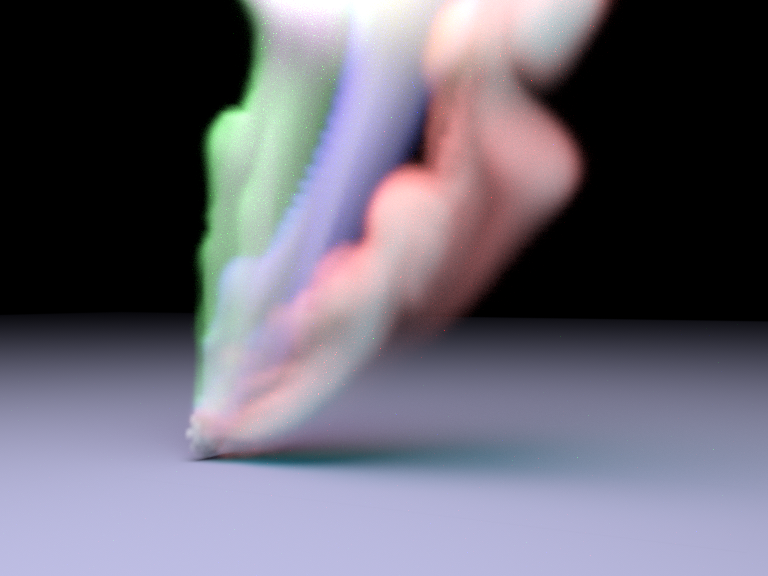
\includegraphics[width=\linewidth]{imgs/colored_smoke.png}
    \caption{A heterogeneous volume with spectrally varying density over space, rendered with multiple-scattering. Smoke data generated using Wenzel Jakob's \href{http://www.mitsuba-renderer.org/misc.html}{fsolver}.}
    \label{fig:gallery}
\end{figure}

In this homework, we will build a volumetric path tracers that can handle scattering and absorption inside participating media inside lajolla. We will split the development into 6 steps and build 6 volumetric path tracers, each has more features than the previous ones.\footnote{This approach is inspired by Steve Marschner's \href{https://www.cs.cornell.edu/courses/cs6630/2015fa/notes/10volpath.pdf}{course note} on volumetric path tracing.} Your $n$-th volumetric path tracer should be able to render all scenes the $(n-1)$-th one can handle. 

Participating media are volumes with many infinitesimal particles absorbing and scattering lights. Given a ray inside the volume parametrized by distance $\mathbf{p}(t)$, the radiance along the ray is modelled by the \emph{radiative transfer equation}:
\begin{equation}
\frac{\mathrm{d}}{\mathrm{d}t} L(\mathbf{p}(t), \omega) = -(\sigma_a(\mathbf{p}(t)) + \sigma_s(\mathbf{p}(t))) L(\mathbf{p}(t), \omega) + \sigma_a L_e(\mathbf{p}(t), \omega) + \sigma_s(\mathbf{p}(t)) \int_{S^2} \rho(\mathbf{p}(t), \omega, \omega') L(\mathbf{p}(t), \omega') \mathrm{d}\omega',
\label{eq:rte}
\end{equation}
where $L$ is the radiance, $\sigma_a$ is the \emph{absorption coefficient}, $\sigma_s$ is the \emph{scattering coefficient}, $L_e$ is the (volumetric) emission, $\rho$ is the \emph{phase function} that is skin to BSDF in surface rendering, and $S^2$ is the spherical domain.

This looks a bit scary, so let's break it down. From now on we'll drop the arguments for $\sigma_a$ and $\sigma_s$, but in general they can still be spatially varying. The radiative transfer equation is made of three components: \textbf{absorption}, \textbf{in-scattering}, and \textbf{out-scattering}. An absorption-only volume contains particles that absorbs energy and light energy is attenuated along the ray
\begin{equation}
\frac{\mathrm{d}}{\mathrm{d}t} L_a(\mathbf{p}(t), \omega) = -\sigma_a L_a(\mathbf{p}(t), \omega) + \sigma_a L_e(\mathbf{p}(t), \omega).
\end{equation}
Notice how this is just a simple linear ordinary differential equation $x' = ax + b$, where $\sigma_a$ attenuates lights and $L_e$ is the gain.

The in-scattering accounts for all the lights bounces between the particles along the ray, just like the surface rendering equation:
\begin{equation}
\frac{\mathrm{d}}{\mathrm{d}t} L_{is}(\mathbf{p}(t), \omega) = \sigma_s \int_{S^2} \rho(\mathbf{p}(t), \omega, \omega') L(\mathbf{p}(t), \omega') \mathrm{d}\omega'.
\end{equation}

However, the light does not just bounce \emph{into} the ray, it also bounces \emph{out}. That's what the out-scattering considers:
\begin{equation}
\frac{\mathrm{d}}{\mathrm{d}t} L_{os}(\mathbf{p}(t), \omega) = -\sigma_s L_{os}(\mathbf{p}(t)).
\end{equation}

Combining all these three components, we get the full radiative transfer equation (Equation~\ref{eq:rte}). Notice that the full radiative transfer equation is also like a linear ODE: $-(\sigma_a + \sigma_s) L$ attenuates light, and $L_e$ and the spherical integral are the gain that makes things brighter.

We'll start from a very simplified version of the radiative transfer equation, then slowly handle more complex situations.

\section{}

\end{document}